\chapter{\todo{Skew Octupolar Fields}}
\label{chapter:skew_octupole_fields}
\thumbforchapter{}
%\chaptertoc{}
%\newpage

\section{\todo{Correction of skew octupole Fields at Top Energy}}

\begin{enumerate}
    \color{red}
    \item RDT Measurements
    \item Orthogonality of correctors
    \item Response Matrix
    \item Correction
    \item Comparison to 2018
\end{enumerate}


\section{\todo{Correction of Skew Octupole Fields at Injection Energy}}

\begin{figure}[H]
    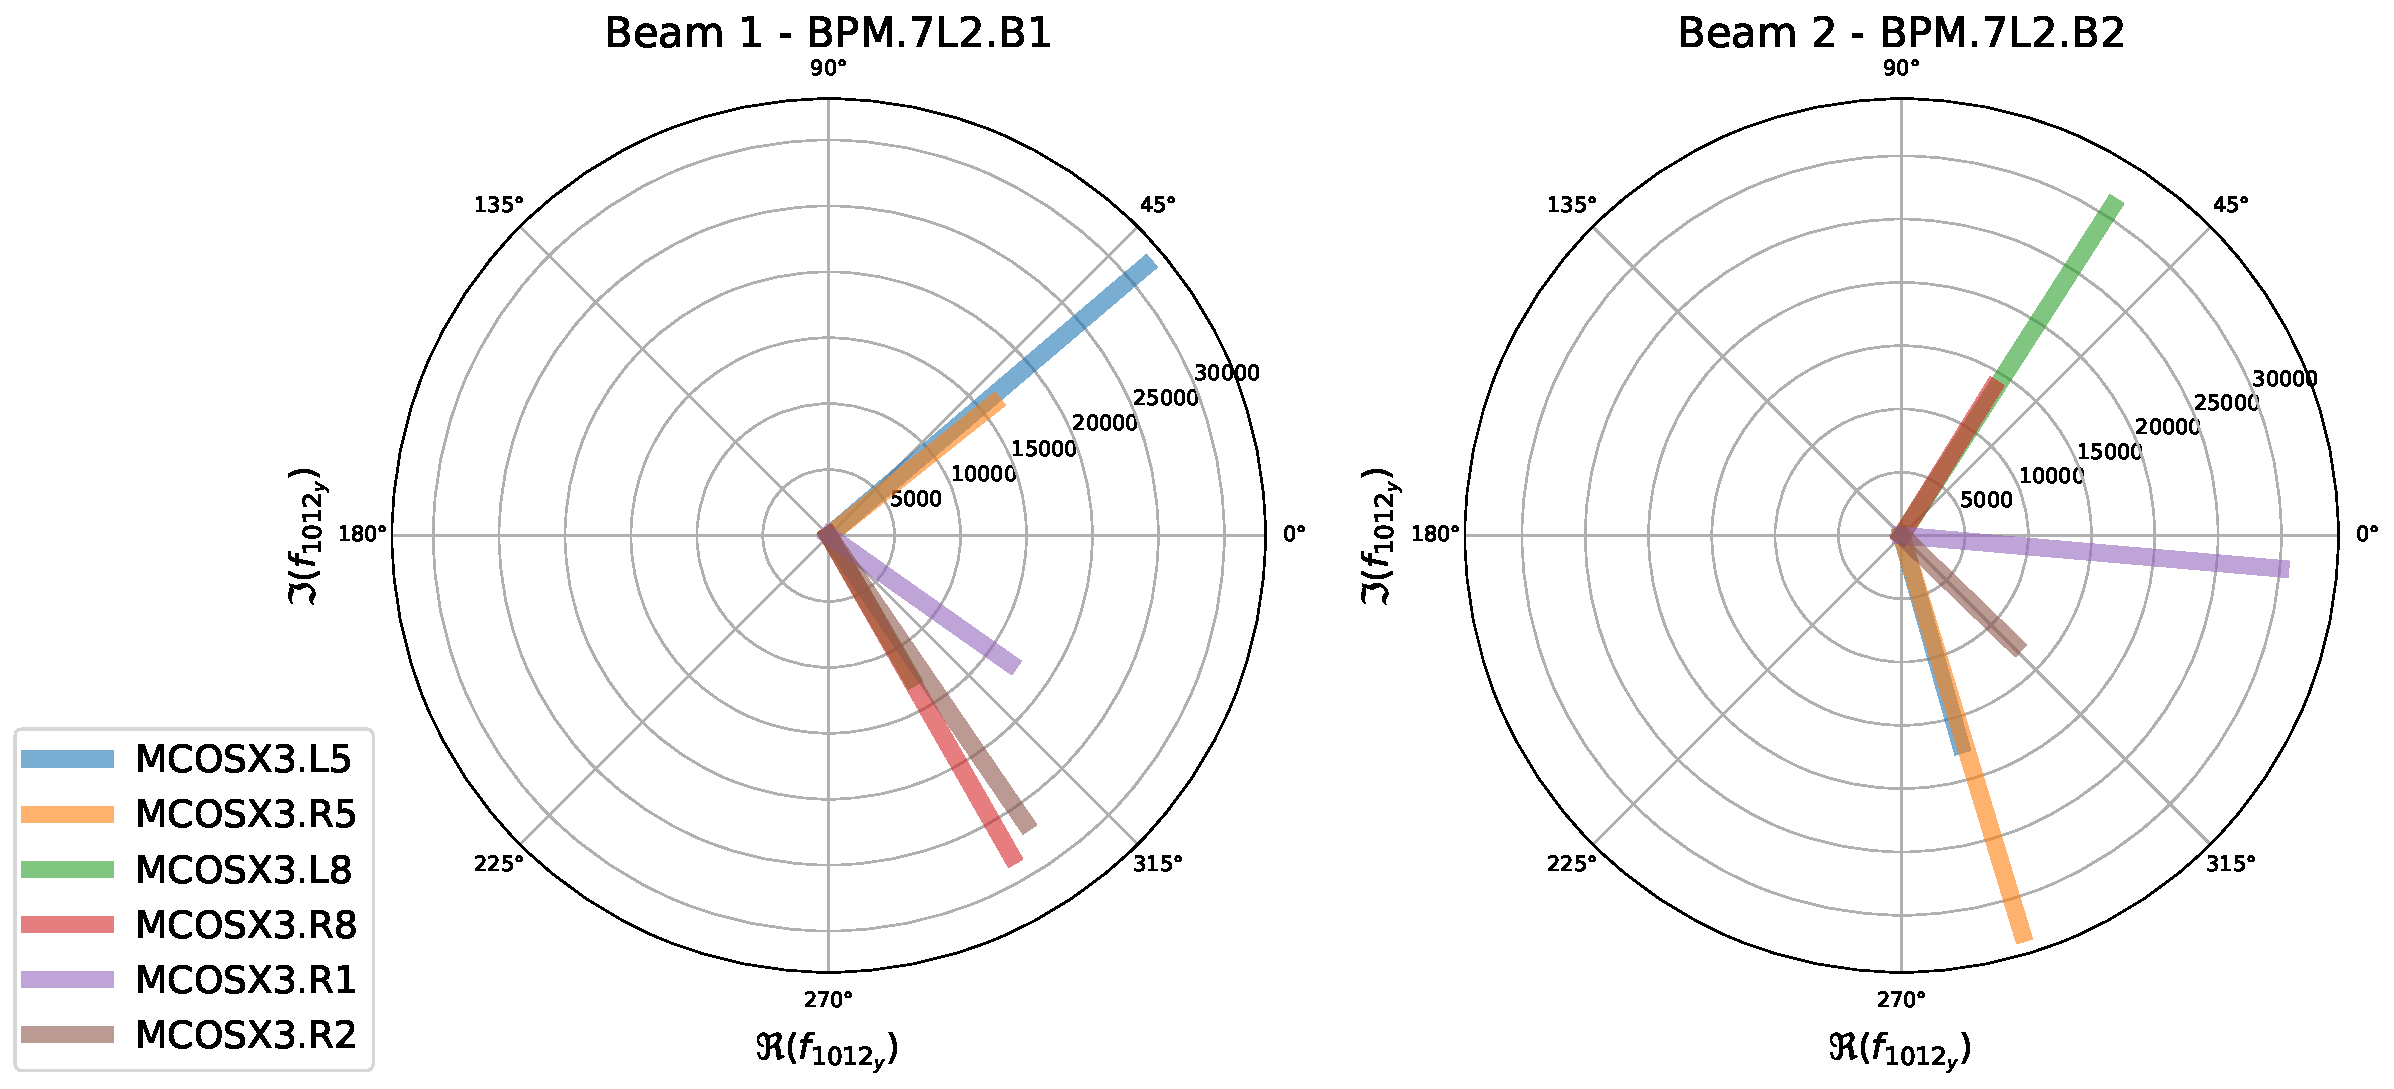
\includegraphics[width=\textwidth]{./chapters/07_octupoles/images/f1012_y_injection.pdf}
    \caption{}
    \label{fig:a4_injection_orthogonal_f1012}
\end{figure}

\begin{figure}[H]
    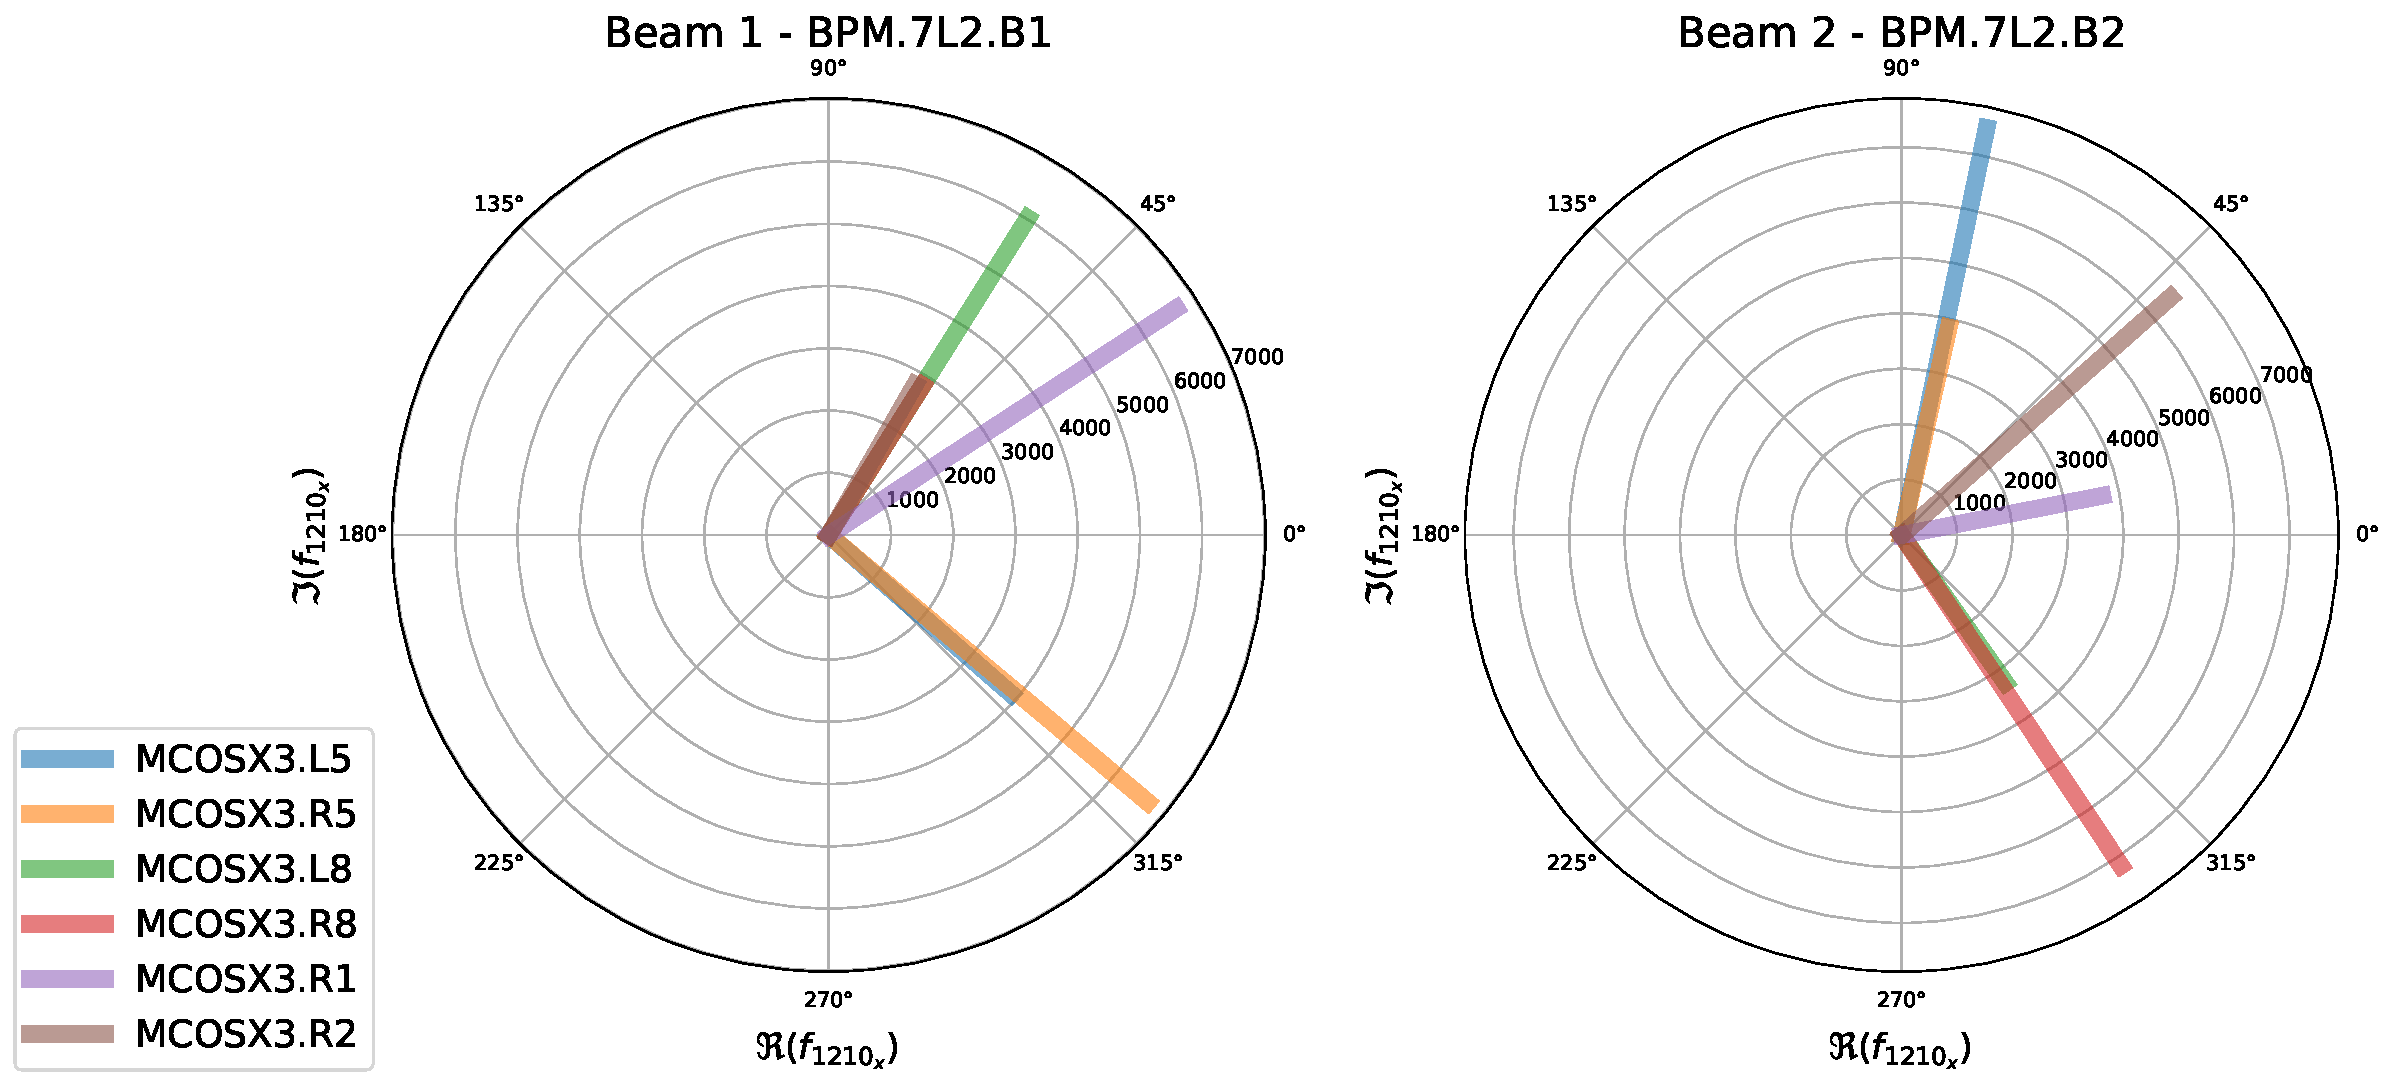
\includegraphics[width=\textwidth]{chapters/07_octupoles/images/f1210_x_injection.pdf}
    \caption{}
    \label{fig:a4_injection_orthogonal_f1210}
\end{figure}





\section{\todo{Skew Octupolar Fields from Landau Octupoles}}